\ProvidesFile{MpM_Manual.tex}

\documentclass[letterpaper,titlepage,twoside]{report}

% Begin Preamble:

%\usepackage[T1]{fontenc}
%\usepackage{palatino}
\usepackage{times}
%\usepackage{bookman}
%\usepackage{newcent}

\usepackage{amsmath}
\usepackage{enumerate}
\usepackage{ifthen}
\usepackage{alltt}
\usepackage{calc}
\usepackage{shortvrb}
\usepackage{varioref}
\usepackage[dvips]{graphicx}
\usepackage[dvips,usenames]{color}
\usepackage{makeidx}
\usepackage{xspace}
\usepackage{fancyhdr}
\usepackage[section]{tocbibind}

% Control the code, depending on whether a hyper-linked PDF is being generated:
\newboolean{generatingHyperPDF}
\setboolean{generatingHyperPDF}{true}

% If the package 'hyperref' is disabled by commenting out the following lines,
% be sure to set the boolean 'generatingHyperPDF' to false.
\ifthenelse{\boolean{generatingHyperPDF}}%
 {\usepackage[dvips,
    colorlinks=true,
    linkcolor=webgreen,
    filecolor=webbrown,
    citecolor=webgreen,
    urlcolor=webblue,
    pdftitle={Movement And Meaning Middleware},
    pdfauthor={Norman Jaffe},
    pdfkeywords={movement,middleware,YARP,ACE,JUCE},
    pdfsubject={Middleware},
    bookmarks,
    raiselinks=true,
    plainpages=false,
    bookmarksopen=true,
    pdfstartview=Fit,
    pdfpagemode=UseOutlines]{hyperref}}
 {\newcommand{\hyperpage}[1]{#1}}

\usepackage{mysects}

% Adjust the paper edges:
\setlength{\parindent}{0em}
\setlength{\textwidth}{\paperwidth-144pt}% 2"
\setlength{\marginparsep}{0pt}
\setlength{\marginparwidth}{0pt}
\setlength{\evensidemargin}{-18pt}% 0.25"
\setlength{\oddsidemargin}{-18pt}% 0.25"

% Some colours for the web:
\definecolor{webgreen}{rgb}{0,0.5,0}
\definecolor{webbrown}{rgb}{0.6,0,0}
\definecolor{webblue}{rgb}{0,0,0.5}

% Define some common strings:
\newcommand{\default}{!-!-!}
\newcommand{\MMM}{Movement~and~Meaning~Middleware}
\newcommand{\mplusm}{\textbf{M+M}}
\newcommand{\nothing}{\ }
\newcommand{\yarp}{\begin{footnotesize}\textsf{YARP}\end{footnotesize}}

% Set up the page layout:
\pagestyle{fancyplain}
\newcommand{\mymark}{}
\lhead[]{\fancyplain{}{\textsc{\mymark}}}
\chead[]{}
\rhead[\fancyplain{}{\textsc{\mymark}}]{}
\lfoot[Page \thepage]{\today}
\cfoot[\MMM]{\MMM}
\rfoot[\today]{Page \thepage}
\renewcommand{\headrulewidth}{0.5bp}
\pagenumbering{roman}

% Set the float behaviour:
\setcounter{bottomnumber}{2}
\setcounter{totalnumber}{4}

% Suppress the normal numbering of sections, et cetera:
\setcounter{secnumdepth}{-3}
\setcounter{tocdepth}{2}

% A couple of useful commands to handle italic-to-normal transitions:
\newcommand{\textitcorr}[1]{\textit{#1}\/}
\newcommand{\emphcorr}[1]{\emph{#1}\/}

% Some commands to make examples match actual output more closely:
\newcommand{\pseudotab}{\thinspace\boldmath{$\vdash$}\thinspace}
\newcommand{\pseudotwotabs}{\thinspace\boldmath{$\vdash$}\thinspace\boldmath{$\vdash$}\thinspace}
\newcommand{\clientName}{\textunderscore{}client\textunderscore{}}
\newcommand{\serviceName}{\textunderscore{}service\textunderscore{}}
\newlength{\utilLen}

\newcommand*{\compLang}[1]{\emphcorr{#1}}

% First argument: index category
% Second argument: index subcategory
% Third argument: alternate index subcategory
% Fourth argument: index name
% Fifth argument: index suffix 
\newcommand{\multiindex}[5]{%
  \ifthenelse{\equal{#2}{\default{}}}%
    {\index{#1!#4#5}}%
    {\index{#1!#2!#4#5}}}

% First argument: label category
% Second argument: label subcategory
% Third argument: alternate label subcategory
% Fourth argument: label name
\newcommand{\multilabel}[4]{%
  \ifthenelse{\equal{#3}{\default{}}}%
    {\label{#1:#4}}%
    {\label{#1:#3:#4}}}

% First argument: reference category
% Second argument: reference subcategory
% Third argument: alternate reference subcategory
% Fourth argument: reference name
\newcommand{\multiref}[4]{%
  \ifthenelse{\equal{#3}{\default{}}}%
    {\ref{#1:#4}}%
    {\ref{#1:#3:#4}}}

% The net effect is as follows:
%  generatingHyperPDF
%   'D' \textitcorr{\color{webgreen}#3}  \hypertarget{hyper.#2.#3}{}\label{#2:#3}  {}
%   'E' {}  {}  {}
%	'M' {} \hypertarget{hyper.#2.#3}{}\label{#2:#3} {}
%   'R' \hyperlink{hyper.#2.#3}{\textitcorr{#3}}  \index{#2!#3}  \ref{#2:#3}
%   'S' \textitcorr{#3}  \index{#2!#3}  {}
%   'X' \hyperlink{hyper.#2.#3}{\textitcorr{#3}}  {}  {}
%  not generatingHyperPDF
%   'D' \textitcorr{\color{webgreen}#3}  \index{#2!#3|(textbf}\label{#2:#3}  {}
%   'E' {}  \index{#2!#3|)textbf}  {}
%   'M' {}  \index{#2!#3|(textbf}\label{#2:#3}  {}
%   'R' \textitcorr{#3}  \index{#2!#3}  \ref{#2:#3}
%   'S' \textitcorr{#3}  \index{#2!#3}  {}
%   'X' \textitcorr{#3}  {}  {}

%   D = Define the object (emphasize the index, create a label);
%   E = End of the object definition (close the index, no text);
%	M = Define the object (no visible text)
%   R = Refer to the object in the index (the default);
%   S = Reference to a standard object and
%   X = Don't add a reference for the object to the index (any letter except D or
%         R could be used, X is preferred for mnemonic value)

% First argument: hyperlink/index category
% Second argument: hyperlink/index subcategory
% Third argument: alternate hyperlink/index subcategory
% Fourth argument: hyperlink/index name
% Fifth argument: alternate hyperlink/index name
\ifthenelse{\boolean{generatingHyperPDF}}%
  {\newcommand{\entityNameD}[5]{%  command if generatingHyperPDF
    \hypertarget{hyper.#1.#4}{}%
	\ifthenelse{\equal{#5}{\default{}}}%
	  {\textitcorr{\color{webgreen}#4}\multiindex{#1}{#2}{#3}{#4}{|(textbf}}%
	  {\textitcorr{\color{webgreen}#5}\multiindex{#1}{#2}{#3}{#5}{|(textbf}}%
    \multilabel{#1}{#2}{#3}{#4}}}
  {\newcommand{\entityNameD}[5]{%  command if not generatingHyperPDF
	\ifthenelse{\equal{#5}{\default{}}}%
	  {\textitcorr{\color{webgreen}#4}\multiindex{#1}{#2}{#3}{#4}{|(textbf}}%
	  {\textitcorr{\color{webgreen}#5}\multiindex{#1}{#2}{#3}{#5}{|(textbf}}%
    \multilabel{#1}{#2}{#3}{#4}}}

% First argument: hyperlink/index category
% Second argument: hyperlink/index subcategory
% Third argument: alternate hyperlink/index subcategory
% Fourth argument: hyperlink/index name
% Fifth argument: alternate hyperlink/index name
\ifthenelse{\boolean{generatingHyperPDF}}%
  {\newcommand{\entityNameE}[5]{}}%
  {\newcommand{\entityNameE}[5]{%
    \ifthenelse{\equal{#1}{#4}}%
    {}% if first and fourth argument match
    {\ifthenelse{\equal{#5}{\default{}}}%
      {\multiindex{#1}{#2}{#3}{#4}{|)textbf}}%
      {\multiindex{#1}{#2}{#3}{#5}{|)textbf}}}}}

% First argument: hyperlink/index category
% Second argument: hyperlink/index subcategory
% Third argument: alternate hyperlink/index subcategory
% Fourth argument: hyperlink/index name
% Fifth argument: alternate hyperlink/index name
\ifthenelse{\boolean{generatingHyperPDF}}%
  {\newcommand{\entityNameM}[5]{%  command if generatingHyperPDF
	\hypertarget{hyper.#1.#4}{}%
	\ifthenelse{\equal{#5}{\default{}}}%
	  {\multiindex{#1}{#2}{#3}{#4}{|(textbf}}%
	  {\multiindex{#1}{#2}{#3}{#5}{|(textbf}}%
  	\multilabel{#1}{#2}{#3}{#4}}}
  {\newcommand{\entityNameM}[5]{%  command if not generatingHyperPDF
	\ifthenelse{\equal{#5}{\default{}}}%
	  {\multiindex{#1}{#2}{#3}{#4}{|(textbf}}%
	  {\multiindex{#1}{#2}{#3}{#5}{|(textbf}}%
    \multilabel{#1}{#2}{#3}{#4}}}

% First argument: hyperlink/index category
% Second argument: hyperlink/index subcategory
% Third argument: alternate hyperlink/index subcategory
% Fourth argument: hyperlink/index name
% Fifth argument: alternate hyperlink/index name
\ifthenelse{\boolean{generatingHyperPDF}}%
  {\newcommand{\entityNameP}[5]{%  command if generatingHyperPDF
    \hypertarget{hyper.#1.#4}{}%
	\ifthenelse{\equal{#5}{\default{}}}%
	  {#4\multiindex{#1}{#2}{#3}{#4}{|(textbf}}%
	  {#5\multiindex{#1}{#2}{#3}{#5}{|(textbf}}%
    \multilabel{#1}{#2}{#3}{#4}}}
  {\newcommand{\entityNameP}[5]{%  command if not generatingHyperPDF
	\ifthenelse{\equal{#5}{\default{}}}%
	  {#4\multiindex{#1}{#2}{#3}{#4}{|(textbf}}%
	  {#5\multiindex{#1}{#2}{#3}{#5}{|(textbf}}%
    \multilabel{#1}{#2}{#3}{#4}}}

% First argument: hyperlink/index category
% Second argument: hyperlink/index subcategory
% Third argument: alternate hyperlink/index subcategory
% Fourth argument: hyperlink/index name
% Fifth argument: alternate hyperlink/index name
\ifthenelse{\boolean{generatingHyperPDF}}%
  {\newcommand{\entityNameR}[5]{%  command if generatingHyperPDF
	\ifthenelse{\equal{#5}{\default{}}}%
	  {\hyperlink{hyper.#1.#4}{\textitcorr{#4}}%
	  \ifthenelse{\equal{#1}{#4}}%
	    {}% if first and fourth argument match
	    {\multiindex{#1}{#2}{#3}{#4}{}}}%
	  {\hyperlink{hyper.#1.#4}{\textitcorr{#5}}%
	  \ifthenelse{\equal{#1}{#4}}%
	    {}% if first and fourth argument match
	    {\multiindex{#1}{#2}{#3}{#5}{}}}%
  	\multiref{#1}{#2}{#3}{#4}}}
  {\newcommand{\entityNameR}[5]{%  command if not generatingHyperPDF
  	\ifthenelse{\equal{#5}{\default{}}}%
	  {\textitcorr{#4}%
	  \ifthenelse{\equal{#1}{#4}}%
	    {}% if first and fourth argument match
	    {\multiindex{#1}{#2}{#3}{#4}{}}}%
	  {\textitcorr{#5}%
	  \ifthenelse{\equal{#1}{#4}}%
	    {}% if first and fourth argument match
	    {\multiindex{#1}{#2}{#3}{#5}{}}}%
    \multiref{#1}{#2}{#3}{#4}}}

% First argument: hyperlink/index category
% Second argument: hyperlink/index subcategory
% Third argument: alternate hyperlink/index subcategory
% Fourth argument: hyperlink/index name
% Fifth argument: alternate hyperlink/index name
\newcommand{\entityNameS}[5]{%
  \ifthenelse{\equal{#5}{\default{}}}%
	{\textitcorr{#4}}%
	{\textitcorr{#5}}%
  \ifthenelse{\equal{#1}{#4}}%
    {}% if first and fourth argument match
    {\multiindex{#1}{#2}{#3}{#4}{}}}

% First argument: hyperlink/index category
% Second argument: hyperlink/index subcategory
% Third argument: alternate hyperlink/index subcategory
% Fourth argument: hyperlink/index name
% Fifth argument: alternate hyperlink/index name
\ifthenelse{\boolean{generatingHyperPDF}}%
  {\newcommand{\entityNameX}[5]{%  command if generatingHyperPDF
	\ifthenelse{\equal{#5}{\default{}}}%
	  {\hyperlink{hyper.#1.#4}{\textitcorr{#4}}}%
	  {\hyperlink{hyper.#1.#5}{\textitcorr{#5}}}}}
  {\newcommand{\entityNameX}[5]{%  command if not generatingHyperPDF
  \ifthenelse{\equal{#5}{\default{}}}%
	{\textitcorr{#4}}%
	{\textitcorr{#5}}}}

% Use \entityReference, rather than \entityName, for the first mention of an object within
% another object, so that page ranges will be present.
\ifthenelse{\boolean{generatingHyperPDF}}%
  {\newcommand{\entityReference}[2]{\entityNameR{#1}{\default{}}{\default{}}{#2}{\default{}}}}%  command if generatingHyperPDF
  {\newcommand{\entityReference}[2]{\entityNameR{#1}{\default{}}{\default{}}{#2}{\default{}} \vpageref[(][(]{#1:#2})}}%  command if not generatingHyperPDF

\ifthenelse{\boolean{generatingHyperPDF}}%
  {\newcommand{\companyReference}[2]{\href{#1}{#2}}}%  command if generatingHyperPDF
  {\newcommand{\companyReference}[2]{#2}}% command if not generatingHyperPDF

% First argument [optional]: alternate name
% Second argument: entity name
\newcommand{\clientNameD}[2][\default{}]{\entityNameD{Clients}{\default{}}{\default{}}{#2}{#1}}% shortcut
\newcommand{\clientNameE}[2][\default{}]{\entityNameE{Clients}{\default{}}{\default{}}{#2}{#1}}% shortcut
\newcommand{\clientNameM}[2][\default{}]{\entityNameM{Clients}{\default{}}{\default{}}{#2}{#1}}% shortcut
\newcommand{\clientNameP}[2][\default{}]{\entityNameP{Clients}{\default{}}{\default{}}{#2}{#1}}% shortcut
\newcommand{\clientNameR}[2][\default{}]{\entityNameR{Clients}{\default{}}{\default{}}{#2}{#1}}% shortcut
\newcommand{\clientNameS}[2][\default{}]{\entityNameS{Clients}{\default{}}{\default{}}{#2}{#1}}% shortcut
\newcommand{\clientNameX}[2][\default{}]{\entityNameX{Clients}{\default{}}{\default{}}{#2}{#1}}% shortcut

% First argument [optional]: alternate name
% Second argument: entity name
\newcommand{\serviceNameD}[2][\default{}]{\entityNameD{Services}{\default{}}{\default{}}{#2}{#1}}% shortcut
\newcommand{\serviceNameE}[2][\default{}]{\entityNameE{Services}{\default{}}{\default{}}{#2}{#1}}% shortcut
\newcommand{\serviceNameM}[2][\default{}]{\entityNameM{Services}{\default{}}{\default{}}{#2}{#1}}% shortcut
\newcommand{\serviceNameP}[2][\default{}]{\entityNameP{Services}{\default{}}{\default{}}{#2}{#1}}% shortcut
\newcommand{\serviceNameR}[2][\default{}]{\entityNameR{Services}{\default{}}{\default{}}{#2}{#1}}% shortcut
\newcommand{\serviceNameS}[2][\default{}]{\entityNameS{Services}{\default{}}{\default{}}{#2}{#1}}% shortcut
\newcommand{\serviceNameX}[2][\default{}]{\entityNameX{Services}{\default{}}{\default{}}{#2}{#1}}% shortcut

\newcommand{\serviceReference}[1]{\entityReference{Services}{#1}}

% First argument [optional]: alternate name
% Second argument: entity name
\newcommand{\utilityNameD}[2][\default{}]{\entityNameD{Utilities}{\default{}}{\default{}}{#2}{#1}}% shortcut
\newcommand{\utilityNameE}[2][\default{}]{\entityNameE{Utilities}{\default{}}{\default{}}{#2}{#1}}% shortcut
\newcommand{\utilityNameM}[2][\default{}]{\entityNameM{Utilities}{\default{}}{\default{}}{#2}{#1}}% shortcut
\newcommand{\utilityNameP}[2][\default{}]{\entityNameP{Utilities}{\default{}}{\default{}}{#2}{#1}}% shortcut
\newcommand{\utilityNameR}[2][\default{}]{\entityNameR{Utilities}{\default{}}{\default{}}{#2}{#1}}% shortcut
\newcommand{\utilityNameS}[2][\default{}]{\entityNameS{Utilities}{\default{}}{\default{}}{#2}{#1}}% shortcut
\newcommand{\utilityNameX}[2][\default{}]{\entityNameX{Utilities}{\default{}}{\default{}}{#2}{#1}}% shortcut

% First argument [optional]: alternate name
% Second argument: Subcategory
% Third argument: entity name
\newcommand{\examplesNameD}[3][\default{}]{\entityNameD{Examples}{#2}{#2}{#3}{#1}}% shortcut
\newcommand{\examplesNameE}[3][\default{}]{\entityNameE{Examples}{#2}{#2}{#3}{#1}}% shortcut
\newcommand{\examplesNameM}[3][\default{}]{\entityNameM{Examples}{#2}{#2}{#3}{#1}}% shortcut
\newcommand{\examplesNameP}[3][\default{}]{\entityNameP{Examples}{#2}{#2}{#3}{#1}}% shortcut
\newcommand{\examplesNameR}[3][\default{}]{\entityNameR{Examples}{#2}{#2}{#3}{#1}}% shortcut
\newcommand{\examplesNameS}[3][\default{}]{\entityNameS{Examples}{#2}{#2}{#3}{#1}}% shortcut
\newcommand{\examplesNameX}[3][\default{}]{\entityNameX{Examples}{#2}{#2}{#3}{#1}}% shortcut

% First argument [optional]: alternate name
% Second argument: Subcategory
% Third argument: Alternate subcategory name
% Fourth argument: entity name
\newcommand{\requestsNameD}[4][\default{}]{\entityNameD{Requests}{#2}{#3}{#4}{#1}}% shortcut
\newcommand{\requestsNameE}[4][\default{}]{\entityNameE{Requests}{#2}{#3}{#4}{#1}}% shortcut
\newcommand{\requestsNameM}[4][\default{}]{\entityNameM{Requests}{#2}{#3}{#4}{#1}}% shortcut
\newcommand{\requestsNameP}[4][\default{}]{\entityNameP{Requests}{#2}{#3}{#4}{#1}}% shortcut
\newcommand{\requestsNameR}[4][\default{}]{\entityNameR{Requests}{#2}{#3}{#4}{#1}}% shortcut
\newcommand{\requestsNameS}[4][\default{}]{\entityNameS{Requests}{#2}{#3}{#4}{#1}}% shortcut
\newcommand{\requestsNameX}[4][\default{}]{\entityNameX{Requests}{#2}{#3}{#4}{#1}}% shortcut

\newcommand*{\insertpart}[2]{\clearpage\renewcommand{\mymark}{#1}#2}

% First argument [optional]: alternate hyperlink name
% Second argument: section title
% Third argument: hyperlink section
% Fourth argument: simplified version of title
% Fifth argument: prefix to display before title
\ifthenelse{\boolean{generatingHyperPDF}}%
  {\newcommand*{\sectionStart}[5][\default{}]{\clearpage\section{#5\texorpdfstring{#2}{#4}}%
   \renewcommand{\mymark}{#4}%
   \ifthenelse{\equal{#1}{\default{}}}%
    {\hypertarget{hyper.#3.#4}{}}%
    {\hypertarget{hyper.#3.#1}{}}}}%
  {\newcommand*{\sectionStart}[5][\default{}]{\clearpage\section{#5#2}\renewcommand{\mymark}{#4}}}

\newcommand*{\sectionEnd}[1]{#1} % just a notational convenience

% First argument: hyperlink section
% Second argument: hyperlink name
% Third argument: simplified version of title
\ifthenelse{\boolean{generatingHyperPDF}}%
  {\newcommand{\sectionRef}[3]{\hyperlink{hyper.#1.#2}{\textitcorr{#3}}}}%
  {\newcommand{\sectionRef}[3]{}}

% First argument: [optional] alternate hypertarget name
% Second argument: subsection title
% Third argument: hypertarget section
% Fourth argument: simplified version of title
\ifthenelse{\boolean{generatingHyperPDF}}%
  {\newcommand*{\subsectionStart}[4][\default{}]{\subsection{\texorpdfstring{#2}{#4}}%
   \ifthenelse{\equal{#1}{\default{}}}%
    {\hypertarget{hyper.#3.#4}{}}%
    {\hypertarget{hyper.#3.#1}{}}}}%
  {\newcommand*{\subsectionStart}[4][\default{}]{\subsection{#2}}}
    
\newcommand*{\subsectionEnd}[1]{#1} % just a notational convenience

% First argument: [optional] alternate hypertarget name
% Second argument: subsubsection title
% Third argument: hypertarget section
% Fourth argument: simplified version of title
\ifthenelse{\boolean{generatingHyperPDF}}%
  {\newcommand*{\subsubsectionStart}[4][\default{}]{\subsubsection{\texorpdfstring{#2}{#4}}%
   \ifthenelse{\equal{#1}{\default{}}}%
    {\hypertarget{hyper.#3.#4}{}}%
    {\hypertarget{hyper.#3.#1}{}}}}%
  {\newcommand*{\subsubsectionStart}[4][\default{}]{\subsubsection{#2}\index{#2}}}
    
\newcommand*{\subsubsectionEnd}[1]{#1} % just a notational convenience

% First argument: [optional] alternate section name
% Second argument: section title
\newcommand*{\primaryStart}[2][\default{}]{%
  \sectionStart[#1]{#2}{Primary}{#2}{}}

\newcommand*{\primaryEnd}[1]{#1} % just a notational convenience

% First argument: subsubsection name
% Second argument: link title
\newcommand{\primaryRef}[2]{\sectionRef{Primary}{#1}{#2}}

% First argument: [optional] alternate subsection name
% Second argument: subsection title
\newcommand*{\secondaryStart}[2][\default{}]{%
  \subsectionStart[#1]{#2}{Secondary}{#2}}

\newcommand*{\secondaryEnd}[1]{#1} % just a notational convenience

% First argument: subsubsection name
% Second argument: link title
\newcommand{\secondaryRef}[2]{\sectionRef{Secondary}{#1}{#2}}

% First argument: [optional] alternate subsubsection name
% Second argument: subsubsection title
\newcommand*{\tertiaryStart}[2][\default{}]{%
  \subsubsectionStart[#1]{#2}{Tertiary}{#2}}

\newcommand*{\tertiaryEnd}[1]{#1} % just a notational convenience

% First argument: subsubsection name
% Second argument: link title
\newcommand{\tertiaryRef}[2]{\sectionRef{Tertiary}{#1}{#2}}

% First argument: [optional] alternate appendix name
% Second argument: appendix title
\newcommand*{\appendixStart}[2][\default{}]{%
  \sectionStart[#1]{#2}{Appendix}{#2}{\appendixname{}:~}}

\newcommand*{\appendixEnd}[1]{#1} % just a notational convenience

% First argument: appendix name
% Second argument: link title
\newcommand{\appendixRef}[2]{\sectionRef{Appendix}{#1}{#2}}

\newenvironment{histList}
  {\begin{list}
    {}
    {\setlength{\labelwidth}{108pt}% 1.5"
    \setlength{\leftmargin}{\labelwidth+\labelsep}
    \setlength{\rightmargin}{36pt}% 0.5"
    \setlength{\parsep}{0ex}
    \renewcommand{\makelabel}[1]{\textbf{##1}\hfill}
    }}
  {\end{list}}
\newcommand*{\histListBegin}{\begin{histList}}
\newcommand*{\histListEnd}{\end{histList}}
\newcommand{\histListItem}[1]{\item[#1]}

\newcommand*{\outputBegin}{\begin{quote}\begin{ttfamily}\begin{small}}
\newcommand*{\outputEnd}{\end{small}\end{ttfamily}\end{quote}}

% Define hyphenation points:

\title{\cal\Huge\textitcorr{\MMM}\\
\vspace{1ex}
\begin{center}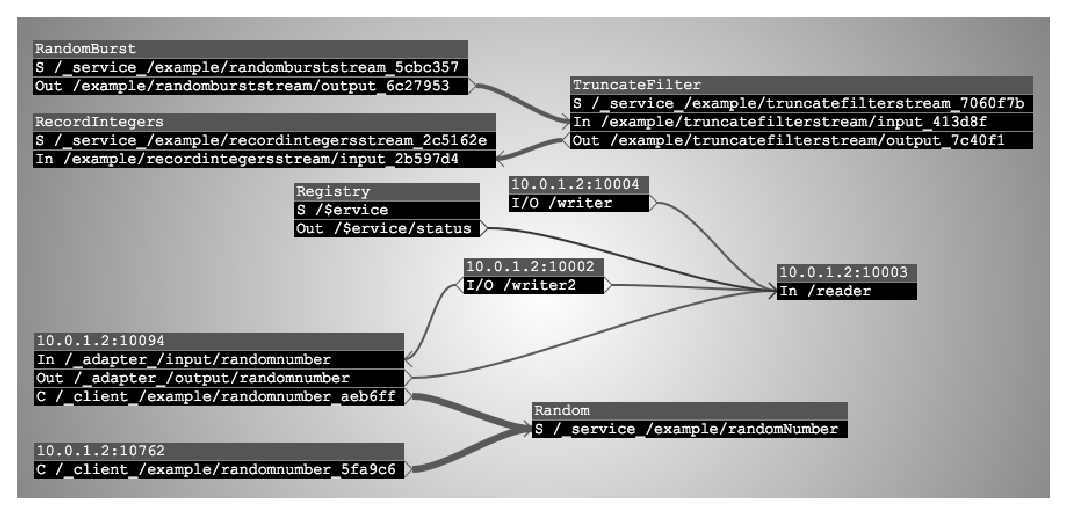
\includegraphics{ChannelManager.eps}\end{center}}
\author{HPlus~Technologies~Ltd. and Simon~Fraser~University\\
Vancouver, British~Columbia, Canada}

\makeindex

%\listfiles
% End Preamble

\begin{document}

% Begin front matter

\maketitle

\insertpart{Contents}{\tableofcontents}
\insertpart{List~of~Figures}{\listoffigures}

\ProvidesFile{documentationHistory.tex}[1.0.0]
\primaryStart[DocumentHistory]{Document~History}
\histListBegin
\histListItem{September 2014}{added description of exemplar classes}
\histListItem{August 2014}{first version of this document}
\histListEnd
\primaryEnd{}
\ProvidesFile{frontispiece.tex}[1.0.0]
\primaryStart{Foreword}
\begin{quote}
\begin{small}
Copyright: \copyright{} 2014 by HPlus~Technologies~Ltd. and Simon~Fraser~University.
\\
All rights reserved. Redistribution and use in source and binary forms, with or without
modification, are permitted provided that the following conditions are met:\\
$\bullet$ Redistributions of source code must retain the above copyright notice, this list
of conditions and the following disclaimer.\\
$\bullet$ Redistributions in binary form must reproduce the above copyright notice, this
list of conditions and the following disclaimer in the documentation and/or other
materials provided with the distribution.\\
$\bullet$ Neither the name of the copyright holders nor the names of its contributors may
be used to endorse or promote products derived from this software without specific prior
written permission.\\
THIS SOFTWARE IS PROVIDED BY THE COPYRIGHT HOLDERS AND CONTRIBUTORS "AS IS" AND ANY
EXPRESS OR IMPLIED WARRANTIES, INCLUDING, BUT NOT LIMITED TO, THE IMPLIED WARRANTIES OF
MERCHANTABILITY AND FITNESS FOR A PARTICULAR PURPOSE ARE DISCLAIMED.
IN NO EVENT SHALL THE COPYRIGHT OWNER OR CONTRIBUTORS BE LIABLE FOR ANY DIRECT, INDIRECT,
INCIDENTAL, SPECIAL, EXEMPLARY, OR CONSEQUENTIAL DAMAGES (INCLUDING, BUT NOT LIMITED TO,
PROCUREMENT OF SUBSTITUTE GOODS OR SERVICES; LOSS OF USE, DATA, OR PROFITS; OR BUSINESS
INTERRUPTION) HOWEVER CAUSED AND ON ANY THEORY OF LIABILITY, WHETHER IN CONTRACT, STRICT
LIABILITY, OR TORT (INCLUDING NEGLIGENCE OR OTHERWISE) ARISING IN ANY WAY OUT OF THE USE
OF THIS SOFTWARE, EVEN IF ADVISED OF THE POSSIBILITY OF SUCH DAMAGE.

Adobe, the Adobe logo, Acrobat, the Acrobat logo, Distiller, Illustrator, Photoshop and
PageMaker are trademarks of
\companyReference{http://www.adobe.com}{Adobe Systems Incorporated}.

Apple, Applescript, Mac, the Mac logo, and Macintosh are trademarks of
\companyReference{http://www.apple.com}{Apple Incorporated}.

dvips(k) copyright \copyright{} 2013
\companyReference{http://www.radicaleye.com}{Radical Eye Software}.

TextWrangler copyright \copyright{}
\companyReference{http://www.barebones.com}{Bare Bones Software Incorporated}.

GPL Ghostscript copyright \copyright{} 2002
\companyReference{http://www.artifex.com}{Artifex Software Incorporated}.

GNU Make copyright \copyright{} 2006
\companyReference{http://www.gnu.org}{Free Software Foundation, Incorporated}.

cmake copyright \copyright{} 2000
\companyReference{http://www.kitware.com}{Kitware Incorporated}.

ACE copyright \copyright{} 1993--2009
\companyReference{http://www.cs.wustl.edu/\%7Eschmidt/ACE.html}{Douglas C. Schmidt}.

YARP copyright \copyright{} 2006
\companyReference{http://wiki.icub.org/yarpdoc/what_is_yarp.html}{RobotCub Consortium}.

JUCE copyright \copyright{} 2013
\companyReference{http://www.juce.com}{Raw Material Software Limited}.

OGDF copyright \copyright{} 2007
\companyReference{http://www.ogdf.net}{Open Graph Drawing Framework}.

MacTeX copyright \copyright{} 2005 \companyReference{https://tug.org/mactex}{MacTeX}.

Leap Motion copyright \copyright{} 2013
\companyReference{https://www.leapmotion.com}{Leap Motion, Incorporated}
\end{small}
\end{quote}
\vspace{\fill}
This document was created using \companyReference{https://tug.org/mactex}{MacTeX}-2014,
\companyReference{http://www.barebones.com}{TextWrangler} 4.5.10,
\companyReference{http://www.artifex.com}{GPL Ghostscript} 9.10,
\companyReference{http://www.gnu.org}{GNU Make version} 3.81,
\companyReference{http://www.tug.org/metapost.html}{MetaPost} 1.902 and
\companyReference{http://www.radicaleye.com}{dvips(k)} 5.994 on an Apple iMac.
\primaryEnd{}
\clearpage\pagenumbering{arabic}

% End of front matter
% Begin contents

\ProvidesFile{overview.tex}[v1.0.0]
\primaryStart{Overview}

\mplusm{} is a software system that acts as an intermediary between subsystems that
provide sensor data, such as accelerometers and motion capture cameras, and actuators
such as projectors and sound systems.
It provides mechanisms for reporting and interrogating the protocols used by the sensors
and actuators, as well as a standard architecture for creating services.

A \mplusm{} installation consists of a set of programs that interconnect using the
\companyReference{http://wiki.icub.org/yarpdoc/what_is_yarp.html}{YARP} networking
protocols, along with libraries that can be linked to applications to provide access to
the \mplusm{} features.

There are three main classes of programs in the set -- services, clients and utilities.
Clients use a formalized protocol to connect to services and utilities manage or monitor
the aggregate state of a \mplusm{} configuration.
There is a unique service, the \serviceNameR[Service~Registry]{ServiceRegistry}, that
maintains information on all the active services that are accessible to clients within a
\mplusm{} installation.
Each service can support multiple client connections, and the client functionality can be
embedded in command--line tools, GUI--based applications or headless background processes.

\primaryEnd{}


\ProvidesFile{utilities.tex}[v1.0.0]
\primaryStart{Utilities}
The utility programs that are provided with \mplusm{} provide access to the processes that
are running in the \mplusm{} installation.
Although command--line \yarp{} commands can also be used to manage the network
connections, it is recommended that the more specialized \mplusm{} tools be used, to avoid
inconsistencies.
\secondaryStart[GUITools]{GUI~Tools}
Currently there is one GUI--based tool, \utilityNameR[Channel~Manager]{ChannelManager},
which provides a view of the state of connections within an \mplusm{} installation, as
well as managing non--\mplusm{} \yarp{} network connections.
\tertiaryStart{\utilityNameP[Channel~Manager]{ChannelManager}}
The \utilityNameX[Channel~Manager]{ChannelManager} application displays a single window
view of the connections within a \yarp{} network, with features designed to make
management of an \mplusm{} installation easier.
Simple \yarp{} network ports are shown as rectangles with a title consisting of the IP
address and port number of the port, and the \yarp{} name for the port as the body of the
rectangle, prefixed with `In' for input--only ports, `Out' for output--only ports and
`I/O' for general ports.\\

\mplusm{} services are shown as rectangles with a title consisting of the name provided by
the service, with the primary \yarp{} network connection as the first row in the body of
the rectangle, prefixed with `S' to indicate that it is a service connection.
Secondary \yarp{} network connections appear as rows below the primary connection,
prefixed with `In' for input--only connections and `Out' for output--only connections.
\mplusm{} \inputOutput{} services do not have a visual appearance that is distinct from
other \mplusm{} services -- the connections that are allowed, however, are more
restricted.
Both \mplusm{} services and clients can have multiple secondary \yarp{} network ports.\\

\mplusm{} simple clients are shown as rectangles with a title consisting of the IP address
and port number of their connection to a service, with a row containing the \yarp{}
network connection prefixed with `C'.\\

\mplusm{} adapters are similar to \mplusm{} simple clients, except that they have
additional rows above the client--service \yarp{} network connection for the secondary
\yarp{} network connections, with prefixes of `In' for input--only connections and `Out'
for output--only connections.\\

Connections between ports are shown as lines with one of three thicknesses and one of
three colours.
The thinnest lines represent simple \yarp{} network connections, which have no explicit
behaviours.
The middle thickness lines represent connections between \inputOutput{} services; these
connections have specific behaviours.
The thickest lines represent connections between clients and services, which are not
modifiable by this tool.
TCP/IP connections, which are the default, are shown in teal, UDP connections are shown in
purple and other connections are shown in orange.
Note that the tool can only create TCP/IP or UDP connections.\\

To create a connection between two ports, click on the source port with the `Option' /
`Alt' key held down and either drag the mouse to the destination port or click on the
destination port.
If the `Shift' is held down at the same time as the `Option' / `Alt' key, the new
network connection will be UDP rather than TCP/IP.
While an `add' operation is active, the source port will be overlaid with a small filled
yellow circle.
To clear a pending `add' operation, either click on the source port a second time or click
somewhere other than a port.
Note that it is not possible to add a connection from an input--only port, from a client
port to a non--service port, or from an output--only port of an \inputOutput{} service to
an input--only port of another \inputOutput{} service if the ports do not have matching
protocols.\\

To remove a connection between two ports, click on the source port with the `Command' key
held down and then click on the destination port.
While a `remove' operation is active, the source port will be overlaid with a small
hollow yellow circle.
To clear a pending `remove' operation, either click on the source port a second time or
click on a port that is not connected to the source port or somewhere other than a port.
Note that is is not possible to remove a connection from a client to a service.\\

If one of the rectangular objects is clicked on with the `Control' key held down, an
information window will be presented.
If the title of the rectangle is clicked on, the information will be about the
object in general while, if a port is clicked on, the information will be about the
specific port.\\

Clicking on a rectangular object with no modifier key held down allows the user to drag
the object around in the window.
Note that connections cannot be selected by clicking on them.\\

The positions of the objects within the window are stored in the file `settings.txt'
within the `ChannelManager' directory inside the user--specific application data
directory.
On Microsoft Windows, this will likely be ``\textbackslash{}Documents~and~Settings%
\textbackslash{}username\textbackslash{}Application~Data'' while, for Macintosh OS X, it
will likely be ``\textasciitilde/Library''.\\

In addition, there are three commands available to alter the display:
\begin{itemize}
\item \textbf{Cmd--B} use a black~/~white background versus a gradient
\item \textbf{Cmd--I} invert the background
\item \textbf{Cmd--R} force a repaint, in case there's a `glitch'
\end{itemize}
\objDiagram{cmDiagram.ps}{cmDiagram}{Channel~Manager structure}
\tertiaryEnd{\utilityNameE[Channel~Manager]{ChannelManager}}
\secondaryEnd{}
\newpage
\secondaryStart[CommandLineUtilities]{Command--Line~Utilities}
\mplusm{} includes a number of command--line tools that provide some of the functionality
of the GUI--based tool, \utilityNameR[Channel~Manager]{ChannelManager}.
As well, the native \yarp{} command--line tools to create and remove connections can be
used with \mplusm{}, but it is very easy to create a non--functional installation if care
is not taken.
\tertiaryStart{\utilityNameP{mpmClientList}}
The program \utilityNameX{mpmClientList} displays the clients for services that have
\yarp{} network connections with persistent state.
A service that has persistent state for its connections retains information from each
request for the following request.
An example service with persistent state is
\examplesNameR{Services}{mpmRunningSumService}, where the information that is kept is the
running sum for the connected client.
The program takes an optional argument for the \yarp{} network port of the service; if no
argument is provided, all services are checked for connections with persistent state.
It has two command--line options:
\begin{itemize}
\item \textbf{--j} generate JSON--formatted output
\item \textbf{--t} generate output in tab--delimited form
\end{itemize}
If neither option is present, the output is written as simple text.\\

The output specifies the \yarp{} network port of a service with persistent state and the
\yarp{} network ports that are connected to it.\\

For example, the default output could be:
\outputBegin{}
Service:\ /\serviceName/examples/runningSum\\
\settowidth{\utilLen}{Service:\ }%
Clients:\\
\hspace*{\utilLen}/\clientName/examples/runningsum\textunderscore{}4896162
\outputEnd{}
or, if JSON--formatted output is requested:
\outputBegin{}
\openSq{} \textbraceleft{} "Service":\ "/\serviceName/examples/runningSum", "Client":\ \\
"/\clientName/examples/runningsum\textunderscore{}4896162" \textbraceright{} \closeSq
\outputEnd{}
or, if tab--delimited output is requested, with tabs shown as
`\texttt{\boldmath{$\vdash$}}':
\outputBegin{}
/\serviceName/examples/runningSum\pseudotab{}%
/\clientName/examples/runningsum\textunderscore{}4896162
\outputEnd{}
Note that, if no clients are found, the JSON--formatted output would be:
\outputBegin{}
\sqPair
\outputEnd{}
while the default output would be:
\outputBegin{}
No client connections found.
\outputEnd{}
and the tab--delimited output would be empty.
If no matching service is found, the default output would be:
\outputBegin{}
No services found.
\outputEnd{}
and the JSON--formatted and tab--delimited outputs would be empty.
\tertiaryEnd{\utilityNameE{mpmClientList}}
\tertiaryStart{\utilityNameP{mpmPortLister}}
The program \utilityNameX{mpmPortLister} displays the active \yarp{} ports and \mplusm{}
entities.
For each \yarp{} port, its role in the \mplusm{} installation is shown as well as any
incoming and outgoing \yarp{} network connections.
The primary port for each active service is identified, as well as the primary port for
each adapter.
It has two command--line options:
\begin{itemize}
\item \textbf{--j} generate JSON--formatted output
\item \textbf{--t} generate output in tab--delimited form
\end{itemize}
If neither option is present, the output is written as simple text.\\

The output specifies the all the active \yarp{} network ports along with their input and
output \yarp{} network ports; regular \yarp{} network ports are tagged as `Standard',
while \mplusm{} adapter ports are tagged as `Adapter', \mplusm{} client ports are tagged
as `Client' and \mplusm{} service ports are tagged as `Service' or `Service registry'.\\

`Standard' ports report their IP address and network port while `Adapter' ports report
the \mplusm{} port of their client application, `Client' ports report their attached
`Adapter' ports, if any are present and `Service' ports report the name of the \mplusm{}
service that they provide.
The connections indicate their direction relative to the \yarp{} network port that is
being listed, along with the \yarp{} network port that is being connected to and the mode
of the connection, such as TCP or UDP.\\

For example, the default output could be:
\outputBegin{}
Ports:\\
\settowidth{\utilLen}{Por}%
/\textdollar{}ervice:\ Service registry port for 'Registry'.\\
\hspace*{\utilLen}No active connections.\\
/\textdollar{}ervice/status:\ Standard port at 10.0.1.2:10008.\\
\hspace*{\utilLen}Output to /reader via UDP.\\
/reader:\ Standard port at 10.0.1.2:10003.\\
\hspace*{\utilLen}Input from /writer2 via TCP.\\
\hspace*{\utilLen}Input from /writer via TCP.\\
\hspace*{\utilLen}Input from /\textdollar{}ervice/status via UDP.\\
/writer:\ Standard port at 10.0.1.2:10002.\\
\hspace*{\utilLen}Output to /reader via TCP.\\
/writer2:\ Standard port at 10.0.1.2:10004.\\
\hspace*{\utilLen}Output to /reader via TCP.
\outputEnd{}
or, if JSON--formatted output is requested:
\outputBegin{}
\openSq{} \textbraceleft{} "PortName":\ "/\textdollar{}ervice",
"PortClass":\ "Service~registry~port~for~'Registry'", "Inputs":\ \sqPair, "Outputs":\
\sqPair{} \textbraceright{}, \textbraceleft{} "PortName":\ "/\textdollar{}ervice/status",
"PortClass":\ \\
"Standard~port~at~10.0.1.2:10008", "Inputs":\ \sqPair, "Outputs":\ \openSq{}
\textbraceleft{} "Port":\ \\
"/reader", "Mode":\ "UDP" \textbraceright{} \closeSq{} \textbraceright{},
\textbraceleft{} "PortName":\ "/reader", "PortClass":\ \\
"Standard~port~at~10.0.1.2:10003", "Inputs":\ \openSq{} \textbraceleft{} "Port":\
"/writer2", "Mode":\ \\
"TCP" \textbraceright{}, \textbraceleft{} "Port":\ "/writer", "Mode":\ "TCP"
\textbraceright, \textbraceleft{} "Port":\ "/\textdollar{}ervice/status",\\
"Mode":\ "UDP" \textbraceright{} \closeSq, "Outputs":\ \sqPair{} \textbraceright,
\textbraceleft{} "PortName":\ "/writer", "PortClass":\ \\
"Standard~port~at~10.0.1.2:10002", "Inputs":\ \sqPair, "Outputs":\ \openSq{}
\textbraceleft{} "Port":\ \\
"/reader", "Mode":\ "TCP" \textbraceright{} \closeSq{} \textbraceright{},
\textbraceleft{} "PortName":\ "/writer2", "PortClass":\ \\
"Standard~port~at~10.0.1.2:10004", "Inputs":\ \sqPair, "Outputs":\ \openSq{}
\textbraceleft{} "Port":\ \\
"/reader", "Mode":\ "TCP" \textbraceright{} \closeSq{} \textbraceright{} \closeSq
\outputEnd{}
or, if tab--delimited output is requested, with tabs shown as
`\texttt{\boldmath{$\vdash$}}':
\outputBegin{}
/\textdollar{}ervice\pseudotab{}Service~registry~port~for~'Registry'\\		
/\textdollar{}ervice/status\pseudotab{}Standard~port~at~10.0.1.2:10008\pseudotab/%
reader~UDP\\
/reader\pseudotab{}Standard~port~at~10.0.1.2:10003\pseudotab/writer2~TCP,
/writer~TCP,\\
\hspace*{2em}/\textdollar{}ervice/status~UDP\\
/writer\pseudotab{}Standard~port~at~10.0.1.2:10002\pseudotab/reader~TCP\\
/writer2\pseudotab{}Standard~port~at~10.0.1.2:10004\pseudotab/reader~TCP
\outputEnd{}
Note that, if no ports are found, the JSON--formatted output would be:
\outputBegin{}
\sqPair
\outputEnd{}
while the default output would be:
\outputBegin{}
Ports:\\
\settowidth{\utilLen}{Por}%
\hspace*{\utilLen}No ports found.
\outputEnd{}
and the tab--delimited output would be empty.
\tertiaryEnd{\utilityNameE{mpmPortLister}}
\tertiaryStart{\utilityNameP{mpmRequestInfo}}
The program \utilityNameX{mpmRequestInfo} displays information on requests for one or more
active services in the \mplusm{} installation.
It lists each request, along with the \yarp{} network port for the service that handles
the request and details about the request.
The program takes two optional arguments for the \yarp{} network port of the service and
the request to get information on; if the request is not specified, all requests for the
given service are shown and, if no port is specified, all requests for all services are
displayed.
It has two command--line options:
\begin{itemize}
\item \textbf{--j} generate JSON--formatted output
\item \textbf{--t} generate output in tab--delimited form
\end{itemize}
If neither option is present, the output is written as simple text.\\

The output consists of the \yarp{} network port that is used by the service, the name of
the request, its version number, a description of the request, including its expected
input and expected output, as well as alternate names for the request and the format of
its inputs and outputs.\\

The input and output formats have a symbolic representation, which is currently used for
descriptive purposes and not actually validated by the services.\\

An `i' represents an integer value, a `d' represents a floating--point (`double') value,
an `n' represents a numeric value (either an integer or a floating--point number), an `s'
represents a string and a `.' represents an arbitrary value.\\

Values can be grouped in lists by being preceded by a `(' and followed by a `)';
concatenation of values indicates sequential appearance of the values.
That is, `sis' indicates a sequence consisting of a string, and integer and another
string.\\

A `:' indicates a key / value pair and a dictionary is indicated by a leading `[' and a
trailing `]'.\\

`?' after an item indicates that the item is optional, `*' indicates that the preceding
item may appear zero or more times and `+' indicates that the preceding item may appear
one or more times.\\

For example, the default output when both the service and the request are specified could
be:
\outputBegin{}
\begin{tabular}{l@{\ }p{12.8cm}}
Service Port:\ & /\textdollar{}ervice\\
Request:\ & register\\
Version:\ & 1.0\\
Details:\ & Register the service and its requests\\
 & Input:\ the channel used by the service\\
 & Output:\ OK or FAILED, with a description of the problem\\
 & encountered\\
Keywords:\ & register add\\
Inputs:\ & s\\
Outputs:\ & s\\
\end{tabular}
\outputEnd{}
or, if JSON--formatted output is requested:
\outputBegin{}
\openSq{} \textbraceleft{} "Port":\ "//\textdollar{}ervice", "Request":\ "register",
"Version":\ "1.0", "Details":\ \\
"Register the service and its requests\textbackslash{}nInput:\ the channel used by the\\
service\textbackslash{}nOutput:\ OK or FAILED, with a description of the problem\\
encountered", "Keywords":\ \openSq{} "register", "add" \closeSq, "Inputs":\ "s",
"Outputs":\ \\
"s" \textbraceright{} \closeSq
\outputEnd{}
or, if tab--delimited output is requested, with tabs shown as
`\texttt{\boldmath{$\vdash$}}':
\outputBegin{}
/\textdollar{}ervice\pseudotab{}register\pseudotab{}1.0\pseudotab{}Register the service
and its requests\textbackslash{}nInput:\ the\\
channel used by the service\textbackslash{}nOutput:\ OK or FAILED, with a description of
the\\
problem encountered\pseudotab{}register add\pseudotab{}s\pseudotab{}s
\outputEnd{}
For the default output, multiple entries will be separated by a blank line; for
tab--delimited output each entry is on a line by itself and for JSON--formatted output,
the entries are objects within an array.
Note that, if no matching request is found, the JSON--formatted output would be:
\outputBegin{}
\sqPair
\outputEnd{}
while the default output would be:
\outputBegin{}
No matching request found.
\outputEnd{}
and the tab--delimited output would be empty.
If no matching service is found, the default output would be:
\outputBegin{}
No services found.
\outputEnd{}
and the JSON--formatted and tab--delimited outputs would be empty.
\tertiaryEnd{\utilityNameE{mpmRequestInfo}}
\tertiaryStart{\utilityNameP{mpmServiceLister}}
The program \utilityNameX{mpmServiceLister} displays the active services in the \mplusm{}
installation.
It lists each service, along with the service description and requests, as well as the
path to the executable for the service and the \yarp{} network ports that the service
provides.
It has two command--line options:
\begin{itemize}
\item \textbf{--j} generate JSON--formatted output
\item \textbf{--t} generate output in tab--delimited form
\end{itemize}
If neither option is present, the output is written as simple text.\\

The output consists of the \yarp{} network port for the service, the `canonical' name of
the service, the kind of service (`Filter', `Input', `Output', `Normal' or `Registry'), a
short description of the service, a short description of the requests supported by the
service, the path to the executable for the service and any secondary input or output
\yarp{} network ports attached to the service.\\

Note that the description of requests supported by the service does not include the
\secondaryRef{BasicRequests}{`basic'} requests handled by all services or, in the case of
\inputOutput{} services, the \secondaryRef{InputOutputRequests}{`input~/~output'}
requests.\\

For each secondary input or output \yarp{} network port, the protocol supported by the
port is shown.
Note that secondary port protocols have no specific format -- they are simple strings that
must match in order for a connection to be established with the port.
By convention, protocol strings can have formats similar to the input and output formats
for requests, but there is no requirement that the protocol strings have any particular
structure.\\

If a protocol is not specified for a secondary input port, then it will accept any data;
if no protocol is specified for a secondary output port, then its output data has no
particular structure and can only be connected to a \yarp{} network port that has no
protocol.
\newpage
For example, the default output could be:
\outputBegin{}
\begin{tabular}{l@{\ }p{12.8cm}}
Services:\ & \\
\\
Service port:\ & /\textdollar{}ervice\\
Service name:\ & Registry\\
Service kind:\ & Registry\\
Description:\ & The Service Registry service\\
Requests:\ & associate - associate a channel with another channel\\
 & disassociate - remove all associations for a channel\\
 & getAssociates - return the associations of a channel\\
 & match - return the channels for services matching the\\
 & criteria provided\\
 & ping - update the last-pinged information for a channel\\
 & or record the information for a service on the given\\
 & channel\\
 & register - record the information for a service on the\\
 & given channel\\
 & unregister - remove the information for a service on the\\
 & given channel\\
Path:\ & \textellipsis/mpmRegistryService\\
Secondary outputs:\ & /\textdollar{}ervice/status\textbraceleft{}protocol=s%
\textbraceright\\
\\
Service port:\ & /\serviceName/examples/randomburst\textunderscore{}5580745\\
Service name:\ & RandomBurst\\
Service kind:\ & Input\\
Description:\ & The random burst input service\\
Requests:\ & \\
Path:\ & \textellipsis/mpmRandomBurstService\\
Secondary outputs:\ & /examples/randomburst/output\textunderscore{}29511ad%
\textbraceleft{}protocol=d+\textbraceright\\
\\
Service port:\ & /\serviceName/examples/recordintegers\textunderscore{}10efc07\\
Service name:\ & RecordIntegers\\
Service kind:\ & Output\\
Description:\ & The record integers output service\\
Requests:\ & \\
Path:\ & \textellipsis/mpmRecordIntegersService\\
Secondary inputs:\ & /examples/recordintegers/input\textunderscore{}5090e26%
\textbraceleft{}protocol=i+\textbraceright\\
\\
Service port:\ & /\serviceName/examples/truncatefilter\textunderscore{}2ee58eb\\
Service name:\ & TruncateFilter\\
Service kind:\ & Filter\\
Description:\ & The truncate filter service\\
Requests:\ & \\
Path:\ & \textellipsis/mpmTruncateFilterService\\
Secondary inputs:\ & /examples/truncatefilter/input\textunderscore{}39b1d9f%
\textbraceleft{}protocol=d+\textbraceright\\
Secondary outputs:\ & /examples/truncatefilter/output\textunderscore{}6a7d189%
\textbraceleft{}protocol=i+\textbraceright
\end{tabular}
\outputEnd{}
\newpage{}
or, if JSON--formatted output is requested:
\outputBegin{}
\openSq{} \textbraceleft{} "ServicePort":\ "/\textdollar{}ervice", "ServiceName":\
"Registry", "ServiceKind":\ \\
"Registry", "Description":\ "The Service Registry service", "Requests":\ \\
"associate - associate a channel with another channel\textbackslash{}ndisassociate - 
remove\\
all associations for a channel\textbackslash{}ngetAssociates - return the associations of
a\\
channel\textbackslash{}nmatch - return the channels for services matching the criteria\\
provided\textbackslash{}nping - update the last-pinged information for a channel or
record\\
the information for a service on the given channel\textbackslash{}nregister - record the\\
information for a service on the given channel\textbackslash{}nunregister - remove the\\
information for a service on the given channel", "Path":\ \\
"\textellipsis/mpmRegistryService", "SecondaryInputs":\ \sqPair, "SecondaryOutputs":\
\openSq{} \textbraceleft\\
"Name":\ "/\textdollar{}ervice/status", "Protocol":\ "s" \textbraceright{} \closeSq{}
\textbraceright, \textbraceleft{} "ServicePort":\ \\
"/\serviceName/examples/randomburst\textunderscore{}5580745", "ServiceName":\ 
"RandomBurst",\\
"ServiceKind":\ "Input", "Description":\ "The random burst input service",\\
"Requests":\ "", "Path":\ "\textellipsis/mpmRandomBurstService",
"SecondaryInputs":\ \\
\sqPair, "SecondaryOutputs":\ \openSq{} \textbraceleft{} "Name":\ \\
"/examples/randomburst/output\textunderscore{}29511ad", "Protocol":\ "d+"
\textbraceright{} \closeSq{} \textbraceright, \textbraceleft\\
"ServicePort":\ "/\serviceName/examples/recordintegers\textunderscore{}10efc07",\\
"ServiceName":\ "RecordIntegers", "ServiceKind":\ "Output", "Description":\ \\
"The record integers output service", "Requests":\ "", "Path":\ \\
"\textellipsis/mpmRecordIntegersService", "SecondaryInputs":\ \openSq{}
\textbraceleft{} "Name":\ \\
"/examples/recordintegers/input\textunderscore{}5090e26", "Protocol":\ "i+"
\textbraceright{} \closeSq,\\
"SecondaryOutputs":\ \sqPair{} \textbraceright, \textbraceleft{} "ServicePort":\ \\
"/\serviceName/examples/truncatefilter\textunderscore{}2ee58eb", "ServiceName":\ \\
"TruncateFilter", "ServiceKind":\ "Filter", "Description":\ "The truncate\\
filter service", "Requests":\ "", "Path":\ \\
"\textellipsis/mpmTruncateFilterService", "SecondaryInputs":\ \openSq{}
\textbraceleft{} "Name":\ \\
"/examples/truncatefilter/input\textunderscore{}39b1d9f", "Protocol":\ "d+"
\textbraceright{} \closeSq,\\
"SecondaryOutputs":\ \openSq{} \textbraceleft{} "Name":\ 
"/examples/truncatefilter/output\textunderscore{}6a7d189",\\
"Protocol":\ "i+" \textbraceright{} \closeSq{} \textbraceright{} \closeSq
\outputEnd{}
or, if tab--delimited output is requested, with tabs shown as
`\texttt{\boldmath{$\vdash$}}':
\outputBegin{}
/\textdollar{}ervice\pseudotab{}Registry\pseudotab{}Registry\pseudotab{}The Service
Registry service\pseudotab{}associate - \\
associate a channel with another channel\textbackslash{}ndisassociate - remove all\\
associations for a channel\textbackslash{}ngetAssociates - return the associations of a\\
channel\textbackslash{}nmatch - return the channels for services matching the criteria\\
provided\textbackslash{}nping - update the last-pinged information for a channel or
record\\
the information for a service on the given channel\textbackslash{}nregister - record the\\
information for a service on the given channel\textbackslash{}nunregister - remove the\\
information for a service on the given channel\pseudotab\textellipsis/%
mpmRegistryService\pseudotwotabs\\
/\textdollar{}ervice/status\textbraceleft{}protocol=s\textbraceright\\

/\serviceName/examples/randomburst\textunderscore{}5580745\pseudotab{}RandomBurst%
\pseudotab{}Input\pseudotab\\
The random burst input service\pseudotwotabs\textellipsis/mpmRandomBurstService%
\pseudotwotabs\\
/examples/randomburst/output\textunderscore{}29511ad\textbraceleft{}protocol=d+%
\textbraceright\\

/\serviceName/examples/recordintegers\textunderscore{}10efc07\pseudotab{}%
RecordIntegers\pseudotab{}Output\pseudotab\\
The record integers output service\pseudotwotabs\textellipsis/%
mpmRecordIntegersService\pseudotab\\
/examples/recordintegers/input\textunderscore{}5090e26\textbraceleft{}%
protocol=i+\textbraceright\\

/\serviceName/examples/truncatefilter\textunderscore{}2ee58eb\pseudotab{}%
TruncateFilter\pseudotab{}Filter\pseudotab\\
The truncate filter service\pseudotwotabs\textellipsis/%
mpmTruncateFilterService\pseudotab\\
/examples/truncatefilter/input\textunderscore{}39b1d9f\textbraceleft{}%
protocol=d+\textbraceright\pseudotab\\
/examples/truncatefilter/output\textunderscore{}6a7d189\textbraceleft{}%
protocol=i+\textbraceright
\outputEnd{}
For clarity, the full paths to the executables have been shortened and blank lines have
been added; in the actual output the paths would be absolute paths and there would be no
blank lines between the output rows.
Note that, if no services are found, the output would be empty.
\tertiaryEnd{\utilityNameE{mpmServiceLister}}
\tertiaryStart{\utilityNameP{mpmVersion}}
The program \utilityNameX{mpmVersion} displays the version numbers for \mplusm{}, \yarp{}
and ACE, the low--level networking layer used by \mplusm{} and \yarp{}.
It has two command--line options:
\begin{itemize}
\item \textbf{--j} generate JSON--formatted output
\item \textbf{--t} generate output in tab--delimited form
\end{itemize}
If neither option is present, the output is written as simple text.\\

For example, the default output could be:
\outputBegin{}
Movement And Meaning Version:\ 1.4.9, YARP Version:\ 2.3.61, ACE Version:\ 6.2.6
\outputEnd{}
or, if JSON--formatted output is requested:
\outputBegin{}
\textbraceleft{} "M+M":\ "1.4.9", "YARP":\ "2.3.61", "ACE":\ "6.2.6" \textbraceright
\outputEnd{}
or, if tab--delimited output is requested, with tabs shown as
`\texttt{\boldmath{$\vdash$}}':
\outputBegin{}
1.4.9\pseudotab{}2.3.61\pseudotab{}6.2.6
\outputEnd{}
\tertiaryEnd{\utilityNameE{mpmVersion}}
\secondaryEnd{}
\newpage
\secondaryStart[UtilityServicesAndClients]{Utility~Services~and~Clients}
\tertiaryStart{\utilityNameP{mpmRequestCounterService}}
The \utilityNameX{mpmRequestCounterService} application is a background service that is
used to determine the average time to send a simple request, process it and return a
response.\\

It responds to the \requestsNameR{Miscellaneous}{Miscellaneous}{resetcounter} and
\requestsNameR{Miscellaneous}{Miscellaneous}{stats} requests sent by the
companion application \utilityNameR{mpmRequestCounterClient} to manage the statistics
that it gathers.\\

Note that only one copy of the \utilityNameX{mpmRequestCounterService} application can be
running at a time in an \mplusm{} installation, due to its fixed \yarp{} network port.
\tertiaryEnd{\utilityNameE{mpmRequestCounterService}}
\tertiaryStart{\utilityNameP{mpmRequestCounterClient}}
The \utilityNameX{mpmRequestCounterClient} application is a command--line tool to
measure the average time to process a simple request.\\

It uses the \requestsNameR{Miscellaneous}{Miscellaneous}{resetcounter} and
\requestsNameR{Miscellaneous}{Miscellaneous}{stats} requests sent to the
\utilityNameR{mpmRequestCounterService} application to gather the statistics, and a
`dummy' request to provide the requests that are being measured.\\

The program has no arguments or options; it asks for the number of requests to send via
the prompt:
\outputBegin{}
How many requests?
\outputEnd{}
Entering a zero value will exit the program.
An example execution of the program, with the \utilityNameR{mpmRequestCounterService}
application running in the background, could be:
\outputBegin{}
How many requests? 10000\\
count = 10000, elapsed time = 2.2 seconds, average time = 0.22 milliseconds.\\
How many requests? 300000\\
count = 300000, elapsed time = 1.20052 minutes, average time = 0.240104 milliseconds.\\
How many requests? 0\\
\outputEnd{}
\tertiaryEnd{\utilityNameE{mpmRequestCounterClient}}
\secondaryEnd{}
\primaryEnd{}


%% section for each of the utilities

\ProvidesFile{services.tex}[v1.0.0]
\startObject{Services and Their Protocols}{Services and Their Protocols}

||TBD TBD TBD||

||/TBD TBD TBD||

\objEnd{}


%% section for each of the core services

\ProvidesFile{examples.tex}[v1.0.0]
\appendixStart{\textitcorr{Examples}}%
The examples that are part of the \mplusm{} set of source files are provided to support
the development of custom applications.
There are example clients, services, adapters as well as examples of the more specialized
Input, Output and Filter services.\\

All the example applications respond to a `HUP' signal and will exit gracefully when one
is sent to them.
\secondaryStart{Example~Services}
The set of example services include a pair of simple services
[\examplesNameR{Services}{mpmEchoService} and
\examplesNameR{Services}{mpmRandomNumberService}], a service with client context
[\examplesNameR{Services}{mpmRunningSumService}] as well as an input service
[\examplesNameR{Services}{mpmRandomBurstService}], an output service
[\examplesNameR{Services}{mpmRecordIntegersService}] and a filter service
[\examplesNameR{Services}{mpmTruncateFilterService}].\\

Note that services normally have no direct interface.
That is, they are `faceless' applications and perform their operations without user
interaction.
\tertiaryStart{\examplesNameP{Services}{mpmEchoService}}
The \examplesNameX{Services}{mpmEchoService} application responds to
\requestsNameR{Miscellaneous}{Miscellaneous}{echo} requests from the
\examplesNameR{Clients}{mpmEchoClient} application; it simply returns any arguments
sent with the request.\\

Note that the application will exit if the
\serviceNameR[Service~Registry]{ServiceRegistry} is not running.\\

The application has two optional arguments -- an alternative endpoint name to be used and
the port number to be used, if a non--default port is desired; the matching client
application does not directly use the endpoint name to establish a connection to the
service.
\tertiaryEnd{\examplesNameE{Services}{mpmEchoService}}
\tertiaryStart{\examplesNameP{Services}{mpmRandomBurstService}}
The \examplesNameX{Services}{mpmRandomBurstService} application is an Input service,
generating a stream of random floating--point values, with a given `burst size' -- the
number of values sent in a group, and a `burst perdiod' -- the number of seconds between
groups.
The application responds to the standard Input service requests and can be used as a
standalone data generator, without the need for a client connection.\\

The \requestsNameR{\inputOutput{}}{InputOutput}{configure} request has two arguments -- a
floating--point value for the `burst period' and an integer value for the `burst size'.
These values will be applied when the output stream is started or restarted.\\

The \requestsNameR{\inputOutput{}}{InputOutput}{restartStreams} request stops and then
starts the output stream.\\

The \requestsNameR{\inputOutput{}}{InputOutput}{startStreams} request starts a random
number generator for the output stream, using the configured `burst period' and
`burst size'.
Once started, the random number generator will send groups of random floating--point
values via the output \yarp{} network connection.\\

The \requestsNameR{\inputOutput{}}{InputOutput}{stopStreams} request stops the random
number generator, which stops the output \yarp{} network connection.\\ 

Note that the application will exit if the
\serviceNameR[Service~Registry]{ServiceRegistry} is not running.\\

The application has two optional arguments -- an alternative endpoint name to be used and
the port number to be used, if a non--default port is desired.\\

The application also has three optional parameters:
\begin{itemize}
\item \textbf{-p:} specifies the burst period, in seconds, to be used. 
\item \textbf{-s:} specifies the burst size to be used.
\item \textbf{-t:} specifies the tag to be used as part of the service name.
\end{itemize}
The tag is added to the standard name of the service, so that more than one copy of the
service can execute -- an \mplusm{} installation can support multiple copies of each
\inputOutput{} service, but the \utilityNameR[Channel~Manager]{ChannelManager}
application cannot display them without a distinguishing `tag'.
If the tag is not specified, the standard name of the service will be used.\\

The other parameters provide the initial burst period and size; if not specified, a burst
period of 1 second and burst size of 1 will be used.
Note that the burst period and size can also be set via commands, if the application is
running from a terminal.\\

If the application is running from a terminal, the following commands are available:
\begin{itemize}
\item \textbf{b:} start the output stream, sending bursts of data of the specified size
and period. 
\item \textbf{c:} configure the service by providing the burst size and period. 
\item \textbf{e:} stop the output stream. 
\item \textbf{q:} quit the application. 
\item \textbf{r:} restart the output stream. 
\end{itemize}
\tertiaryEnd{\examplesNameE{Services}{mpmRandomBurstService}}
\tertiaryStart{\examplesNameP{Services}{mpmRandomNumberService}}
The \examplesNameX{Services}{mpmRandomNumberService} application responds to
\requestsNameR{Examples}{Examples}{random} requests from the
\examplesNameR{Clients}{mpmRandomNumberClient} application; it simply returns any arguments
sent with the request.\\

Note that the application will exit if the
\serviceNameR[Service~Registry]{ServiceRegistry} is not running.\\

The application has two optional arguments -- an alternative endpoint name to be used and
the port number to be used, if a non--default port is desired; the matching client
application does not directly use the endpoint name to establish a connection to the
service.\\

The \requestsNameD{Examples}{Examples}{random} request has an argument of the
count of floating--point random numbers to be returned as a response to the request.
\requestsNameE{Examples}{Examples}{random}%
\tertiaryEnd{\examplesNameE{Services}{mpmRandomNumberService}}
\tertiaryStart{\examplesNameP{Services}{mpmRecordIntegersService}}
The \examplesNameX{Services}{mpmRecordIntegersService} application is an Output
service, recording a stream of integer values to an external file.
The application responds to the standard Output service requests and can be used as a
standalone data generator, without the need for a client connection.\\

The \requestsNameR{\inputOutput{}}{InputOutput}{configure} request has a single argument,
the file--system path to use for the output file.
The path will be used when the input stream is started or restarted.\\

The \requestsNameR{\inputOutput{}}{InputOutput}{restartStreams} request stops and then
starts the input stream.\\

The \requestsNameR{\inputOutput{}}{InputOutput}{startStreams} request opens a file to be
used for output, using the configured output file path.\\

The \requestsNameR{\inputOutput{}}{InputOutput}{stopStreams} request closes the output
file that is being used.\\

Note that the application will exit if the
\serviceNameR[Service~Registry]{ServiceRegistry} is not running.\\

The application has two optional arguments -- an alternative endpoint name to be used and
the port number to be used, if a non--default port is desired.\\

The application also has two optional parameter:
\begin{itemize}
\item \textbf{-p:} specifies the output file path to be used. 
\item \textbf{-t:} specifies the tag to be used as part of the service name.
\end{itemize}
The tag is added to the standard name of the service, so that more than one copy of the
service can execute -- an \mplusm{} installation can support multiple copies of each
\inputOutput{} service, but the \utilityNameR[Channel~Manager]{ChannelManager}
application cannot display them without a distinguishing `tag'.
If the tag is not specified, the standard name of the service will be used.\\

The output file path parameter provides the initial output file path; if not specified, a
random path in the temporary directory will be used.
For Microsoft Windows, the temporary directory being used is ``\textbackslash{}tmp''
while, for Macintosh OS X, it will be ``/tmp''.
Note that the output file path can also be set via commands, if the application is
running from a terminal.\\

If the application is running from a terminal, the following commands are available:
\begin{itemize}
\item \textbf{b:} start the input stream, using the specified output file path to record
the input data. 
\item \textbf{c:} configure the service by providing the output file path to be used. 
\item \textbf{e:} stop the input stream, which will close the output file. 
\item \textbf{q:} quit the application. 
\item \textbf{r:} restart the input stream, which will cause the current output file to be
closed and a new output file to be opened. 
\end{itemize}
\tertiaryEnd{\examplesNameE{Services}{mpmRecordIntegersService}}
\tertiaryStart{\examplesNameP{Services}{mpmRunningSumService}}
The \examplesNameX{Services}{mpmRunningSumService} application responds to
requests from the \examplesNameR{Clients}{mpmRunningSumClient} application or\\
\examplesNameR{Adapters}{mpmRunningSumAdapter} or
\examplesNameR{Adapters}{mpmRunningSumAltAdapter} adapters; it returns the running sum
associated with the requesting application or adapter.\\

Note that the application will exit if the
\serviceNameR[Service~Registry]{ServiceRegistry} is not running.\\

The application has two optional arguments -- an alternative endpoint name to be used and
the port number to be used, if a non--default port is desired; the matching client
application does not directly use the endpoint name to establish a connection to the
service.\\

The \requestsNameD{Examples}{Examples}{addtosum} request updates the running sum
corresponding to the requesting application or adapter and returns the resulting value.
Note that an \requestsNameX{Examples}{Examples}{addtosum} request implicitly starts the
calculation.\\
\requestsNameE{Examples}{Examples}{addtosum}%

The \requestsNameD{Examples}{Examples}{resetsum} request clears the running sum
corresponding to the requesting application or adapter.\\
\requestsNameE{Examples}{Examples}{resetsum}%

The \requestsNameD{Examples}{Examples}{startsum} request starts the running sum
calculation for the requesting application or adapter.
Note that a \requestsNameX{Examples}{Examples}{startsum} request implicitly resets the
calculation, if it has already been started.\\
\requestsNameE{Examples}{Examples}{startsum}%

The \requestsNameD{Examples}{Examples}{stopsum} request stops the running sum
calculation for the requesting application or adapter.
\requestsNameE{Examples}{Examples}{stopsum}%
\tertiaryEnd{\examplesNameE{Services}{mpmRunningSumService}}
\tertiaryStart{\examplesNameP{Services}{mpmTruncateFilterService}}
The \examplesNameX{Services}{mpmTruncateFilterService} application is a Filter
service, converting a stream of floating--point values into a stream of integers.
The application responds to the standard Filter service requests and can be used as a
standalone data generator, without the need for a client connection.\\

The \requestsNameR{\inputOutput{}}{InputOutput}{configure} request has no arguments and
does nothing.\\

The \requestsNameR{\inputOutput{}}{InputOutput}{restartStreams} request stops and then
starts the input and output streams.\\

The \requestsNameR{\inputOutput{}}{InputOutput}{startStreams} request initiates listening
on the input stream; the output stream is only written to when input is seen, so nothing
special is done with it.\\

The \requestsNameR{\inputOutput{}}{InputOutput}{stopStreams} request terminates listening
on the input stream, which will cause sending on the output stream to cease as well.\\

Note that the application will exit if the
\serviceNameR[Service~Registry]{ServiceRegistry} is not running.\\

The application has two optional arguments -- an alternative endpoint name to be used and
the port number to be used, if a non--default port is desired.\\

The application also has one optional parameters:
\begin{itemize}
\item \textbf{-t:} specifies the tag to be used as part of the service name.
\end{itemize}
The tag is added to the standard name of the service, so that more than one copy of the
service can execute -- an \mplusm{} installation can support multiple copies of each
\inputOutput{} service, but the \utilityNameR[Channel~Manager]{ChannelManager}
application cannot display them without a distinguishing `tag'.\\

If the application is running from a terminal, the following commands are available:
\begin{itemize}
\item \textbf{b:} start the input and output streams. 
\item \textbf{c:} configure the service; this has no effect, as the service has no
configurable parameters. 
\item \textbf{e:} stop the input and output streams. 
\item \textbf{q:} quit the application. 
\item \textbf{r:} restart the input and output streams. 
\end{itemize}
\tertiaryEnd{\examplesNameE{Services}{mpmTruncateFilterService}}
\secondaryEnd{}
\secondaryStart{Example~Clients}
The example client applications provided use simple terminal--based interfaces to
generate requests for their matching service applications.
\tertiaryStart{\examplesNameP{Clients}{mpmEchoClient}}
The \examplesNameX{Clients}{mpmEchoClient} application reads input from a terminal and
sends it to the \examplesNameR{Services}{mpmEchoService} application using an
\requestsNameR{Miscellaneous}{Miscellaneous}{echo} request; it exits when an empty line is
entered.
Note that the application will also exit if the
\serviceNameR[Service~Registry]{ServiceRegistry} or the
\examplesNameR{Services}{mpmEchoService} application are not running or if the application
is not running from an interactive terminal.
\tertiaryEnd{\examplesNameE{Clients}{mpmEchoClient}}
\tertiaryStart{\examplesNameP{Clients}{mpmRandomNumberClient}}
The \examplesNameX{Clients}{mpmRandomNumberClient} application reads the count of
random numbers desired from a terminal and sends a
\requestsNameR{Examples}{Examples}{random} request to the
\examplesNameR{Services}{mpmRandomNumberService} application; it exits when a zero is
entered for the count of random numbers desired.
Note that the application will also exit if the
\serviceNameR[Service~Registry]{ServiceRegistry} or the
\examplesNameR{Services}{mpmRandomNumberService} application are not running or if the
application is not running from an interactive terminal.
\tertiaryEnd{\examplesNameE{Clients}{mpmRandomNumberClient}}
\tertiaryStart{\examplesNameP{Clients}{mpmRunningSumClient}}
The \examplesNameX{Clients}{mpmRunningSumClient} application reads commands from a
terminal and sends corresponding requests to the
\examplesNameR{Services}{mpmRunningSumService} application.\\

The commands are:
\begin{itemize}
\item \textbf{+:} read a number from the terminal and send it to the service via an
\requestsNameR{Examples}{Examples}{addtosum} request, to update the running sum for this
client.
\item \textbf{r:} send a \requestsNameR{Examples}{Examples}{resetsum} request to the
service so that it will reset the running sum for this client.
\item \textbf{s:} send a \requestsNameR{Examples}{Examples}{startsum} request to the
service so that it will start calculating the running sum for this client.
\item \textbf{x:} send a \requestsNameR{Examples}{Examples}{stopsum} request to the
service so that it will stop calculating the running sum for this client and then exit the
application.
\end{itemize}
Note that the application will also exit if the
\serviceNameR[Service~Registry]{ServiceRegistry} or the
\examplesNameR{Services}{mpmRunningSumService} application are not running or if the
application is not running from an interactive terminal.
\tertiaryEnd{\examplesNameE{Clients}{mpmRunningSumClient}}
\secondaryEnd{}
\secondaryStart{Example~Adapters}
Adapters are applications that use a client object to connect to an \mplusm{} service,
routing input from one or more input \yarp{} network connection via the client object to
the service and returning results from the client to one or more output \yarp{} network
connections.\\

The example adapters demonstrate using a single input \yarp{} network connection
[\examplesNameR{Adapters}{mpmRandomNumberAdapter} and
\examplesNameR{Adapters}{mpmRunningSumAltAdapter}] or multiple input \yarp{} network
connections [\examplesNameR{Adapters}{mpmRunningSumAdapter}].\\

Note that adapters normally have no direct interface.
That is, they are `faceless' applications and perform their operations without user
interaction.
\tertiaryStart{\examplesNameP{Adapters}{mpmRandomNumberAdapter}}
The \examplesNameX{Adapters}{mpmRandomNumberAdapter} application reads the count of
random numbers desired from an input \yarp{} network connection and sends a
\requestsNameR{Examples}{Examples}{random} request to the
\examplesNameR{Services}{mpmRandomNumberService} application.
The random numbers returned from the service are sent out an output \yarp{} network
connection.
Note that the application will also exit if the
\serviceNameR[Service~Registry]{ServiceRegistry} or the
\examplesNameR{Services}{mpmRandomNumberService} application are not running.
\tertiaryEnd{\examplesNameE{Adapters}{mpmRandomNumberAdapter}}
\tertiaryStart{\examplesNameP{Adapters}{mpmRunningSumAdapter}}

The \examplesNameX{Adapters}{mpmRunningSumAdapter} application reads  values from an input
`data' \yarp{} network connection and commands from an input `control' \yarp{} network
connection and sends corresponding requests to the
\examplesNameR{Services}{mpmRunningSumService} application.\\

If a numeric value is read from the `data' input \yarp{} network connection, it is sent to
the service via an \requestsNameR{Examples}{Examples}{addtosum} request, to update the
running sum for this adapter.
If a string is read from the `control' input \yarp{} network connection, is is considered
to be one of the following commands:
\begin{itemize}
\item \textbf{q:} exit the application.
\item \textbf{r:} send a \requestsNameR{Examples}{Examples}{resetsum} request to the
service so that it will reset the running sum for this adapter.
\item \textbf{s:} send a \requestsNameR{Examples}{Examples}{startsum} request to the
service so that it will start calculating the running sum for this adapter.
\item \textbf{x:} send a \requestsNameR{Examples}{Examples}{stopsum} request to the
service so that it will stop calculating the running sum for this adapter.
\end{itemize}
The running sums returned from the service are sent out an output \yarp{} network
connection.\\

Note that the application will also exit if the
\serviceNameR[Service~Registry]{ServiceRegistry} or the
\examplesNameR{Services}{mpmRunningSumService} application are not running.
\tertiaryEnd{\examplesNameE{Adapters}{mpmRunningSumAdapter}}
\tertiaryStart{\examplesNameP{Adapters}{mpmRunningSumAltAdapter}}
The \examplesNameX{Adapters}{mpmRunningSumAltAdapter} application reads  values and
commands from an input \yarp{} network connection and sends corresponding requests to the
\examplesNameR{Services}{mpmRunningSumService} application.\\

If a numeric value is read from the input \yarp{} network connection, it is sent to the
service via an \requestsNameR{Examples}{Examples}{addtosum} request, to update the running
sum for this adapter.
If a string is read from the input \yarp{} network connection, is is considered to be one
of the following commands:
\begin{itemize}
\item \textbf{q:} exit the application.
\item \textbf{r:} send a \requestsNameR{Examples}{Examples}{resetsum} request to the
service so that it will reset the running sum for this adapter.
\item \textbf{s:} send a \requestsNameR{Examples}{Examples}{startsum} request to the
service so that it will start calculating the running sum for this adapter.
\item \textbf{x:} send a \requestsNameR{Examples}{Examples}{stopsum} request to the
service so that it will stop calculating the running sum for this adapter.
\end{itemize}
The running sums returned from the service are sent out an output \yarp{} network
connection.\\

Note that the application will also exit if the
\serviceNameR[Service~Registry]{ServiceRegistry} or the
\examplesNameR{Services}{mpmRunningSumService} application are not running.
\tertiaryEnd{\examplesNameE{Adapters}{mpmRunningSumAltAdapter}}
\secondaryEnd{}
\appendixEnd{}


%% section for each of the examples

\ProvidesFile{classes.tex}[v1.0.0]
\primaryStart{Classes~and~Their~Interfaces}

			||TBD TBD TBD||

			||/TBD TBD TBD||

\primaryEnd{}


%% section for each of the core classes

\appendix

\ProvidesFile{internalDb.tex}[v1.0.0]
\appendixStart[Internal~Database~Structure]{\textitcorr{Internal~Database~Structure}}%

			||TBD TBD TBD||

			||/TBD TBD TBD||

\appendixEnd{}

\ProvidesFile{registrationSequence.tex}[v1.0.0]
\appendixStart[RegistrationSequence]{\textitcorr{Registration~Sequence}}%

			||TBD TBD TBD||

			||/TBD TBD TBD||

\appendixEnd{}


% End of contents

\insertpart{Index}{\printindex}
\end{document}
\end
